% =========================================================================
% CHAPTER 5
% =========================================================================

\chapter{Implementierung}
\label{K5}
\section{Deployment}
\begin{wrapfigure}{r}{0.4\textwidth}
  \vspace{-23pt}
  \begin{center}
    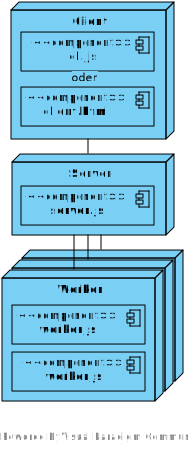
\includegraphics[width=0.275\textwidth]{deploy}
    \caption{UML Deployment Struktur mit Netzwerk Verbindungen.}
    \label{fig:deploy}
  \end{center}
  \vspace{-23pt}
\end{wrapfigure}

Um Komponenten ausführen zu können muss \node{} installiert, und  \cmd{npm install} zum installieren von Third-party Abhängigkeiten verwendet werden.
Das Projekt hat folgende Ordnerstruktur:

\BCL
  \setlength\itemsep{0.0em}
  \item[\footnotesize{\faFolderOpen}] data \dotfill An verteiltes Dateisystem gebunden
  \item[\footnotesize{\faFolderOpen}] doc \hfill
  \item[\footnotesize{\faFolderOpen}] jobScripts \dotfill Benutzerdefinierte Scripts
  \item[\footnotesize{\faFolderOpen}] src \hfill
  \BCL
    \item[\footnotesize{\faFile}] app.js \dotfill Initialisierung und Model
    \item[\footnotesize{\faFile}] config.js \dotfill Konstanten
    \item[\footnotesize{\faFolderOpen}] job \dotfill Middleware API Library
    \item[\footnotesize{\faFolderOpen}] networks \hfill
    \item[\footnotesize{\faFolderOpen}] views \hfill
  \ECL
  \item[\footnotesize{\faFile}] server.js \dotfill \cmd{node worker.js} startet einen Server
  \item[\footnotesize{\faFile}] worker.js \dotfill \cmd{node worker.js} startet einen Worker
  \item[\footnotesize{\faFile}] client.html \hfill
  \item[\footnotesize{\faFile}] cli.js \dotfill \cmd{node cli.js jobscript.js} führt \textit{jobscript} aus
\ECL

\noindent Die System besteht aus mehreren ausführbaren Komponenten:
Der Server \file{server.js}, die Worker \file{worker.js}, der Webclient \file{client.html} sofern der Server läuft, und der CLI-Client \file{cli.js} (siehe Abbildung \ref{fig:deploy}).
Bis auf den Webclient sind sie alle als Node.js Script startbar.
Im Folgenden werden Instanzen dieser als Node bezeichnet.
Der CLI-Client erwartet ein auszuführendes \jobScript{} als Argument.
Die Gemeinsamkeiten dieser ausführbaren Komponenten werden in Abschnitt \ref{app} beschrieben.

Die Unterschied dieser Komponenten sind gering:
CLI-Client und Webclient unterscheiden sich von den anderen Komponenten nur durch das zusätzlich enthaltene \UI{}.
Die Worker unterscheiden sich vom Server nur dadurch, dass sie ClientWebSockets anstatt ServerWebsockts verwenden.
Dieses Design wurde gewählt, um zukünfigte arbeiten mit \ptp{} und \hcsno{} mit mehreren Server und Worker Ebenen zu erleichtern.
Der \file{src/networks/} Ordner könnte mehrere Network Implementierungen enthalten, dezeit ist aber nur eine \hcsno{} Implementierung mit einer Worker Ebene vorhanden.
Das Network Interface wird in \ref{NetworkInterface} beschieben.

Der \file{src/job/} Ordner enthält Libary Code.
Dieser wird bei der Implementierung von \jobScript s benötigt.
Enthalten sind die Job Klasse, Workflow Logic Implementierungen, die \remoteJob{} Klasse und Adapter Jobs \cite{Gamma05a} für standard Technologien wie AJAX und das Betriebsystem Prozess API.


















\clearpage
\section{Globale Objekte und deren Initialisierung}
\label{globals}
Der Browser bzw. \node{} laden zuerst \file{src/app.js}, eines der Netzwerke aus \file{src/networks/} und optional ein \UI{} aus \file{src/views/}.
Ist der Ladevorgang abgeschlossen aktiviert die Initialisierungsfunktion \method{app.init} die geladenen Konponenten in folgenden Schritten:
\BCL
  \item[1.] Konstanten aus \file{src/config.js} werden ins Model übernommen
  \item[2.] Network Events werden an app gebunden (siehe \ref{NetworkInterface})
  \item[3.] Network \method{connect(ipEndpoint)} wird ausgefüht, die eigene Node Info an den Server gesendet, und der Server antwortet mit den Node Infos aller anderen Nodes.
        Der Endpoint wird aus app.config genommen.
  \item[4.] Es werden Timer gestartet um \netInfo{} aktuell zu halten (siehe \ref{netInfo})
  \item[5.] Eine Liste der am Server verfügbaren \jobScript{}  wird geladen
  \item[6.] Der CLI-Client führt an dieser Stelle das als Argument gegebene \jobScript{} aus
  \item[6.] Der Webclient bindet \GUI{} Elemente an das Model
\ECL

\subsection{View}
Views sind optional. CLI- sowie Webclient \UI{} Elemente implementieren das selbe Interface.
Dieses besteht nur aus einer \method{update(diff)} Funktion.
Das Argument \object{diff} enthält neue, gelöschte und geänderte Teile des Models.
Die update Funktionen werden ausschießlich von Model \event{onChange} Events aufgerufen.


\subsection{Network}
\label{NetworkInterface}
Die geladenen Netzwerke sind zunächst passiv. Sie stellen folgendes Interface zur Verfügung:
\BCL
  \item Die \method{connect(ipEndpoint)} Funktion initialisiert aktiv eine Verbindung
  \item Das \event{onConnect(netInfoDiff)} Event wird ausgelöst wenn eine Verbindung aufgebaut wurde
  \item Das \event{onDisconnect(netInfoDiff)} Event wird ausgelöst wenn eine Verbindung terminiert
  \item Das \event{onMessage(data)} Event wird ausgelöst wenn eine Message empfangen wird
  %\item Die bei Verbindungsänderungen übergebenen \object{netInfoDiff} Objekte werden mit der \method{Mergable.update} Funktion ins Model eingepflegt.
\ECL

\subsection{App}
\label{app}
Wird eine Message empfangen, wird zunächst der zugehörige Job anhand der JobID und der RunningJobs Lookup Table ermittelt, und danach die durch die Message definierte Transition ausgefüht.
Die Job Event Funktionen modifizieren dabei das Model (siehe Tabelle \ref{tab1}).
App enthält auch das Model welches sich aus \class{Mergeable} Komponenten zusammensetzt.
Diese werden ausschließlich mit ihrer \method{update(diff)} Funktion modifiziert, und lösen dabei ihr \event{onChange} Event aus.
Damit kann das \UI{} aktuell gehalten werden.
Das Model setzt sich aus folgenden \class{Mergeable} Komponenten zusammen:

%onMessage
%Job.onUpdate | Job.onReturn
%model.update
%view.update

\begin{multicols}{2}

\subsubsection{Config}
Enthält Konstanten aus \file{src/config.js}, erweitert diese mit der Mergable Funktionalität um an das \UI{} gebunden werden zu können.

\subsubsection{\jobScript s}
Enthält eine Liste der am Server bekannten \jobScript s. Die Script Inhalte werden erst bei Zugriff geladen.
Jede \UI{} Action erstellt einen Job basierend auf dem im \jobScript{} definirten Prototypen.

\subsubsection{RunningJobs Lookup Table}
RunningJobs ist eine Liste aller Jobs die auf dem Gerät gerade ausgefüghrt werden, und aller noch laufenden \remoteJob s die auf diesem erstellt wurden.
Sie ist zu Beginn leer, \TransCall s tragen Jobs ein, \TransReturn s entfernen sie.

\subsubsection{\netInfo{}}
\label{netInfo}
Als member des globalen Models, steht diese Komponente in allen Modulen zur Verfügung, auch in \jobScript s.
Das \netInfo{} Objekt wird in \jobScript s verwendet um geeignete Worker auszuwählen.
Es besteht aus einer Liste der im System vorhandenen Nodes.
Jede Node darin bietet folgende Members:
\BCL
  \setlength\itemsep{0.0em}
  \item Funktionen zum Empfangen und Senden
  \item Momentane CPU- und Speicherauslastung
  \item Informationen über das Betriebssystem
  \item Liste der auf der Node installierten Interpreter
\ECL
\noindent \netInfo{} ist zu Beginn leer, und wird durch Network Events \event{onConnect} und \event{onDisconnect} sowie zyklischen Messages aktuell gehalten.
Worker senden zyklisch ihre \netInfo{} Struktur an den Server.
Das ist ausreichend um das \netInfo{} Model am Server aufzubauen.
Der Server sendet zyklisch die akkumulierten Änderungen an die Clients.



\end{multicols}
\begin{wrapfigure}{r}{1\textwidth}
  \begin{center}
    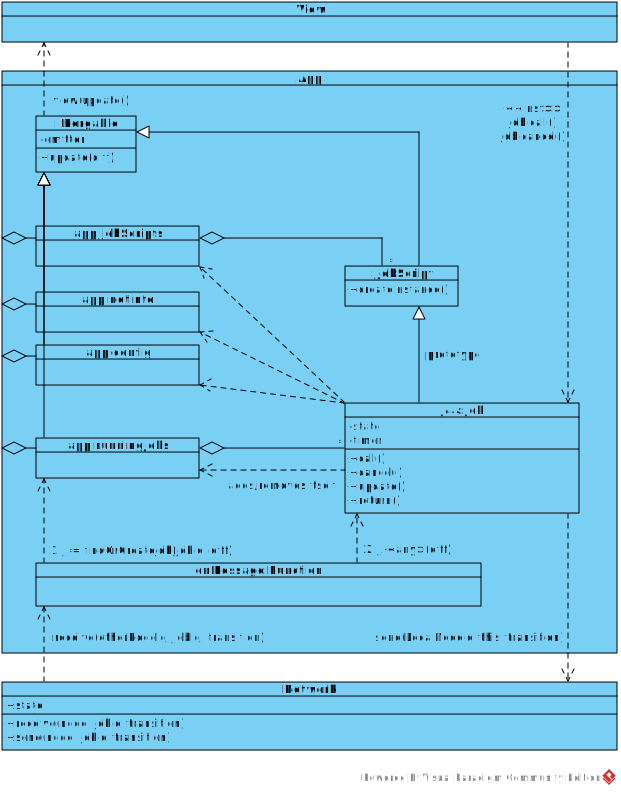
\includegraphics[width=0.9\textwidth]{vm}
  \end{center}
  \label{deploy}
  \label{viewModel}
  \caption{UML Object Diagramm des Client. Server and Worker enthalten keine View. }
\end{wrapfigure}



















\clearpage
\section{Job API}
\label{JobInterface}
\begin{wrapfigure}{r}[10mm]{0.45\textwidth}
  \vspace{-10mm}

  \begin{center}
    \fvset{frame=single,framesep=0mm,fontsize=\small,fontfamily=courier,numbers=left,xleftmargin=5mm,xrightmargin=10mm,framerule=.1mm,numbersep=1mm}
    %\hspace{-5cm}
    \begin{Verbatim}

  var j = new Job({
    params:{},
    onCall:  j=> {
      // calculate something
      j.update(0.5, 'half done')
      // calculate result
      j.return('ok', 'done')
    },
    onUpdate:j=> print(j.output)
    onReturn:j=> print(j.output)
  })
  j.call()

    \end{Verbatim}
  \end{center}
  \caption{Erstellen und starten eines \textcolor{White}{- - -} \protect\linebreak einfachen lokalen Jobs.}
  \label{codejob}
\end{wrapfigure}





Die zentrale Klasse des Middleware API ist die \class{Job} Klasse.
Zu finden in \file{src/job/}.
Sie deckt die Funktionalität von \JavaScript Promises ab, und erweitert diese um Abbrechbarkeit und optionale Zwischenergebnisse.
Jeder Job kann mit einem Timeout versehen werden, dies erleichtert die Implementierung vom \remoteJob s, und kann auch bei lokalen Jobs hilfreich sein.

Die abstrakte Job Klasse implementiert die in Kapitel \ref{jfsm} beschriebene State Machine.
Für den Anwender bedeutet dies, dass sie nicht erlaubte Transitions abfängt.
State Transitions werden mit den Funktionen call, cancel, update und return ausgelöst.
Zu jeder Transition kann der Anwender eine Funktion definieren, die mit der Transition ausgeführt wird.
Im Folgenden werden diese Funktionen Job Event genannt.
Die Implementierungen  dieser Funktionen werden an den Job Konstruktor übergeben.
OnCall muss definiert werden, onCancel, onUpdate und onReturn sind optional (siehe Abbildung \ref{codejob}).


Die bei JavaScript Promises an den Konstruktor übergebene Funktion entspricht dem onCall Event des Jobs.
Die Job.return Funktion übernimmt die Aufgaben der reject und resolve Funktionen von Promises.
onCancel und onUpdate existieren bei JavaScript Promises nicht, da diese nicht abbrechbar sind und keine Zwischenergebnisse liefern können.

Jeder Job muss terminieren, ähnlich wie Promises mit reject oder resolve es tun.
Es gibt vier Arten wie eine onCall Implementierung dies tun kann:
Durch einen Aufruf der Job.return Funktion,
eine Exception,
ein Timeout,
oder durch binden des Jobs an SubJobs mit Hilfe der Job.delegate Funktion (siehe \ref{delegate}, \ref{hfsm}).
Verwendet man Job.onReturn kann neben dem Ergebnisszustand auch ein Ergebnisswert mitgegeben werden.
Für die Übergabe von Zwischenergebnissen und den Progress wird Job.update beliebig oft verwendet.
Ist der Job an SubJobs gebunden, wird Job.return von der Workflow Logic aufgerufen.

\newcommand{\specialcell}[2][c]{%
  \begin{tabular}[#1]{@{}l@{}}#2\end{tabular}}

\begin{table}[H]
\centering
\begin{tabular}[t]{|l|l|l|l|}
\hline
Event Auslöser \ref{JobInterface}                                              & Message (nur bei \remoteJob s) \ref{messages} & Transition \ref{jfsm}    & Job Event Funktion \ref{JobInterface}   \\ \hline
\JobCall (args)                                                                & Call    & call           & Job.onCall(param)$^1$     \\ \hline
\JobCancel ()                                                                  & Cancel  & cancel         & Job.onCancel()         \\ \hline
\JobUpdate (p, d)                                                              & Update  & update         & Job.onUpdate(p, d)     \\ \hline
\JobReturn ('ok', rv)                                                          & Return  & returnOk       & Job.onReturn(s, rv)    \\ \hline
\JobReturn ('canceled')                                                        & Return  & returnCanceled & Job.onReturn(s)    \\ \hline
\specialcell[t, l]{\JobReturn ('fail', e) $\lor$ \\Exception $\lor$ \\Timeout} & Return & returnFailed & Job.onReturn(s, e) \\ \hline
\end{tabular}
\caption{Links: Die vom Anwender aufgerufen Steuerfunktionen, rechts die vom Anwender definierten Event Handler.
         Nur \remoteJob s verwenden Messages. Transitions lösen Job Events aus. \protect\linebreak
         $^1$ obligates Konstruktor Argument der Job Klasse.}
\label{tab1}
\end{table}


























\section{Vorgefertigte Jobs}
%\subsection{\remoteJob{}, \AjaxJob{} und \OsProcessJob{}}

Die in \ref{JobInterface} beschriebene Job Klasse ist abstrakt und dafür vorgesehen vom Anwender spezialisiert zu werden.
Dieser Abschnitt beschreibt drei in der Middleware enthaltenen Spezialisierungen.

\begin{multicols}{3}
\subsection{\remoteJob{}}
\remoteJob s führen die onCall und onCancel Funktion auf einem Remote Gerät aus.
Dem Konstruktor wird eine Node aus dem \netInfo{} Objekt übergeben welche definiert wo sie ausgeführt werden.

\subsection{\AjaxJob{}}
Adaptiert XMLHttpRequest damit dieser in \JobTree s eingesetzt werden kann. OnCall löst den Request aus. ReadyState 1 bis 3 löst update Events aus, ReadyState 4 das onReturn Event \cite{w3cX}.

\subsection{\OsProcessJob{}}
Adaptiert das \node{} Prozess Interface, damit OS-Prozesse in \JobTree s eingesetzt werden können. OnCall startet den Prozess, onCancel sendet ein SIGTERM. Stdout wird auf Job.update umgeleitet.
\end{multicols}



\section{Implementierung von \jobScript s mit \JobTree s}
\label{delegate}

\begin{wrapfigure}{r}[10mm]{0.73\textwidth}
  \vspace{-10mm}

  \begin{center}
    \fvset{frame=single,framesep=0mm,fontsize=\small,fontfamily=courier,numbers=left,xleftmargin=5mm,xrightmargin=10mm,framerule=.1mm,numbersep=1mm,commandchars=\\\{\},codes={\catcode`$=3\catcode`^=7\catcode`_=8}}
    \hspace{-5cm}
    \begin{Verbatim}

\textcolor{BlueViolet}{  onCall: \textbf{j=>} j.delegate(\{}
\textcolor{BlueViolet}{      type: 'toOne',}
\textcolor{BlueViolet}{      job: ()=> \textbf{new RemoteJob}(\{}
\textcolor{BlueViolet}{          desc: 'init workers on server',}
\textcolor{BlueViolet}{          node: app.netInfo.server,}
\textcolor{BlueViolet}{          args: j.params,}
\textcolor{BlueViolet}{          onCall:}\textcolor{OliveGreen}{ \textbf{js=>} js.delegate(\{}
\textcolor{OliveGreen}{              type: 'pool',}
\textcolor{OliveGreen}{              workerPool: app.netInfo.filter('POSIX64'),}
\textcolor{OliveGreen}{              jobCount: 20,}
\textcolor{OliveGreen}{              job: (idx, poolNode)=> \textbf{new RemoteJob}(\{}
\textcolor{OliveGreen}{                  desc: 'empty job on worker',}
\textcolor{OliveGreen}{                  node: poolNode,}
\textcolor{OliveGreen}{                  args: \{\},}
\textcolor{OliveGreen}{                  onCall:}\textcolor{Mahogany}{ \textbf{jw=>} jw.ret('ok', 'no result')}
\textcolor{OliveGreen}{              \})}
\textcolor{OliveGreen}{          \})}
\textcolor{BlueViolet}{      \})}
\textcolor{BlueViolet}{  \})}

    \end{Verbatim}
  \end{center}
  \caption{Ein Pseudo \jobScript{} das 20 leere Jobs auf Workern ausführt. \textcolor{White}{- - -} \protect\linebreak Blau: Client, Grün: Server, Rot: Worker.}
  \label{code}
\end{wrapfigure}

\noindent \jobScript s werden im \textbf{src/jobScripts} Ordner abgelegt.
Der RootJob wird immer vom \UI{} erzeugt.
\jobScript s enthalten nur die onCall Funktion eines Jobs und optional default parameter.
Das \UI{} definiert die onUpdate und onReturn Funktionen, um Ergebniszustand und Daten anzuzeigen.


Abbildung \ref{code} zeigt ein Script, dass 20 ‘leere’ Jobs auf Worker Nodes ausführt.
Die Skript Funktion enthält Code von Client, Server und Worker.
Das onCall Event erhält den \RootJob{} \object{j} als parameter.
Er wird nicht direkt abgearbeitet, sondern an einen \remoteJob{} auf dem Server delegiert.
\method{j.delegate} bindet den Erfolgszustand von \object{j} an den des \remoteJob s \object{js} mit Hilfe der toOne Workflow Logik.
Anders betrachtet fügt es Knoten in den \JobTree{} ein.
Derzeit unterstützt \method{Job.delegate} folgende Workflows:
toOne,
parallel,
pool und
konsekutiv.
Bis auf toOne fügen alle anderen Workflows mehrere Knoten hinzu.
Deshalb ist das \object{job} Argument der delegate Funktion als Factory Method \cite{Gamma05a} ausgeführt.

Es ist nicht verpflichtend wie in diesem Beispiel durchgängig \remoteJob s zu verwenden.
Sie sollten nur Anwendung finden wenn es notwendig ist auf ein anderes Gerät zu wechseln.
Das onCall Event von \remoteJob s wird auf der Node ausgefürt die im Konstruktor spezifiziert wurde.
\remoteJob s bilden im Code Geräteübergänge.
Abbildung \ref{code} zeigt Farblich auf welchen Geräten der Code ausgefürt wird, und nicht die Jobgrenzen.

Man beachte, dass \method{js.delegate} am Server einen Pool Workflow verwendet, also mehrere WorkerJobs (zugleich \remoteJob s in \ref{code}) ausgeführt werden, die sich nur durch ihre Node und Parameter unterscheiden.
\ref{code} Zeile 10

\begin{wrapfigure}{L}{0.6\textwidth}
  \begin{center}
    \includegraphics[width=0.6\textwidth]{tree1}
  \end{center}
  \caption{Screenshot der \JobTree{} Visualisierung des Webclients.
    Jeder Knoten ist ein Job. Grün zeigt den Endzustand Ok an.
    Der gezeigte \JobTree{} wurde mit dem Script aus Abbildung \ref{code} erzeugt.
    \textbf{Oben}: Der am Client vom \UI{} erzeugte \RootJob{} (blau in Abbildung \ref{code}).
    \textbf{Mitte}: Der am Client erzeugte, und am Server ausgeführte \remoteJob{} (grün in Abbildung \ref{code}).
    \textbf{Unten}: Die am Server erzeugten, und auf den Workern ausgeführten \remoteJob s (rot in Abbildung \ref{code}.)}
  \label{fsm0}
  \vspace{22pt}
\end{wrapfigure}

\noindent  zeigt die Auswahl der Worker die den Pool bilden.
\method{netInfo.filter} ist eine Funktion die alle 64bit Posix kompatiblen Nodes aus der \netInfo{} Datenstruktur liefert.
\object{jw} Terminiert bei diesem einfachen Beispiel unmittelbar nach dem Start.
Realistischere Beispiele binden an dieser Stelle einen \OsProcessJob{} ein, oder implementieren einen Nutzlast Algorithmus direskt in JavaScript.

Verwendet man \method{Job.delegate}, kann die Middleware Meta Informationen über den Ablauf (\JobTree s) sammeln.
Die in den folgenden Kapiteln gezeigten Visualisierungen basiren auf \JobTree s.
